%%This is a very basic article template.
%%There is just one section and two subsections.
\documentclass[11pt,a4paper,oneside,twocolumn]{article}
%\documentclass[11pt,a4paper,oneside]{report}

\usepackage{enumerate}
\usepackage{amssymb,amsmath}

\usepackage{graphicx}  
\newcommand{\fig}[1]{\textit{Figure~\ref{#1}}}

\author{Rafael Luiz Klaser, Gustavo Pessin\\
LRM - Laborat\'orio de Rob\'otica M\'ovel\\
Instituto de Ci\^encias Matem\'aticas e de Computa\c{c}\~ao\\
USP / S\~ao Carlos\\
\texttt{rlklaser@icmc.usb.br, pessin@gmail.com}
}

\title{Technical Report \\ Wi-fi Signal strength as fitness for robot navigation}

\begin{document}

\maketitle
%\setcounter{chapter}{1}
%\chapter{I}
\section*{Resume}
%\begin{abstract}

We present here a navigation approach based on the signal strength in wireless
communication between a base station and the moving objects. Our intention is to
be minimalistic as we focus on a robot swarm. 

%We used the signal strenght in a
%wi-fi communication system to lead a vehicle to reach a target goal.

\section{Motivation}

In a robot swarm is desirable that each unit be simple and even disposable. This
leads to simple devices with limited sensors, preferably low cost ones. Some
algorithms for navigation uses the concept of function optimization by computing
a fitness value that leads to a target location. Most fitness functions are
based on testing solutions where the input sometimes in practice is not easy to
provide. This difficulty can be by the lack of the necessary sensory information
but the impossibility to get it ahead of time without a real move of the
vehicle. We want to demonstrate that the signal strength of a wi-fi radio can be
used as a source of fitness.

\section{Background}

As stated in [1], three different categories can be used to classify the
interaction of robots in a swarm : through the environment, through sensing and
through communication. A communication interaction can be performed in a robot
swarm with a wi-fi infrastructure. In a radio based signal transmission the
power and antenna gain are know and the propagation of the signal can be
estimated based on the wavelength, distance and some environment factors.

In radio communication, the propagation loss of the signal is an important
measure to build networks. Propagation and prediction models for indoor local
area networks can be seen in the ITU-R P.1238 recommendation [2]. That guide
provides models that can be used to simulate the signal strength in a coverage
area for indoor wi-fi network. The basic signal loss model presented in [2] is
defined as:

\[L_{total}=20 log_{10}f + N log_{10}d + Lf(n) - 28\]

where:\\
\\
N : distance power loss coefficient;\\
f : frequency (MHz);\\
d : separation distance (m) between the base station and portable terminal (where $d > 1m$);\\
Lf : floor penetration loss factor (dB);\\
n : number of floors between base station and portable terminal ($n \geq 1$).\\


Wi-fi communication between robots and with a base station is common in an
indoor scenario. Another common sensors present in terrestrial robotic
vehicles are wheel's encoders. The wheel encoder allows to estimate the odometry
of the vehicle by dead-reckoning. This kind of odometry is known to have a good
local estimation but drifts over time [3].

\section{Methodology}

% Our simulated robot is equiped whit wheels encoders that we use to estimate
% the odometry by dead-reckoning.
We are using a physical simulation environment for experimental purpose and the
vehicles are built as nonholonomic car-like robot that can only move forward as
it models our desired scenario. Our simulated robot is equipped with a wi-fi
antenna and wheel encoders. This leads to a minimalist equipment well suited to
indoor robot swarm. The odometry is only necessary to move the robot by small
distances each step so the drift is not a concern. The target of each unit is to
reach the base station where the access point is installed. Based on the signal
strength between the robot wi-fi radio and the base station radio we then
estimate a relative distance to the target.

All the robotic simulation and implementation is based on the
ROS\footnote{http://ros.org} (Robotic Operation System) and the network and
radio signal simulation is based on the NS-3\footnote{http://www.nsnam.org}
(Network Simulator) environment.

\section{Beacon Navigation}

The implemented navigation algorithm have the only goal in mind to be simple and
to demonstrate the approach based on the signal strength to reach a target.
The completeness of the algorithm is reached by applying a circular moving
pattern to explore all possible poses of the robot to a base antenna. The ray of
the circular path must be a distance empirically measured that improves the
signal and the turn must comply with the vehicle's kinematics constraints.
The best signal spot is stored with the odometry coordinates then the vehicle
constantly moves to the best position and performs a news circular search. In
practice the robot drifts and looses its orientation to the base because the
signal can be improved in any pose when omnidirectional antennas are used. The
circular exploration leads to a rough path but guaranties somehow that the robot
searches constantly the space for a signal improvement. An example of this
behavior is depicted in \fig{fig:path}.

\begin{figure}[ht]
% \centering
	\begin{minipage}[b]{1\linewidth}
	    \centering
	    \includegraphics[width=\textwidth,height=6cm]{beacon.png}
	 	\caption{Trajectory path - the circles is the commanded moves: a)Source, 
	 	b)Target (antenna), c)Circular search behavior, d)Signal gain attraction spots.}
	 	\label{fig:path}
	\end{minipage}
\end{figure}

\section{Results}

We performed the simulation with a very basic motion planning algorithm based on
circular moves to search for a signal loss reduction. At each signal gain
improvement another circular path is performed around that best signal spot until
the signal strength raises a level that the robot is close enough to the
target.

\section{Conclusions and future work}

In simulations we were able to conduct a robot based on the signal strength of a
wireless communication radio. The next steps is to do implementations of more
efficient algorithms based on this approach and perform experiments in real
scenarios.

\section{References}

[1] Holland, O., ; Melhuish, C.: Stigmergy, Self-organization, and sorting in
collective robotics. Artificial Life 5(2): 173-202. 1999.
\\
{} [2] ITU-R, Propagation data and prediction methods for the planning of
indoor radiocommunication systems and radio local area networks in the frequency
range 900 MHz to 100 GHz, ITU-R P.1238-7, P-Series, Radiowave propagation, 2012.
\\
{} [3] Wolf et al., Rob\'otica m\'ovel inteligente: Da simula\c{c}\~ao 
\`as aplica\c{c}\~oes no mundo real. In: Mini-Curso: Jornada de Atualiza\c{c}\~ao 
em Inform\'atica (JAI), Congresso da SBC. [S.l.: s.n.], 2009.

\end{document}

